\chapter{Other Tools}

\section{Sensitivity Export}
\label{sec:fepest:sensitivity}

Linear sensitivity indicates how strong a parameter influences certain observations. These derivatives are calculated during the optimization and contained in the Jacobian matrix.

The sensitivities are therefore a potentially valuable by-product of the optimization, and can as such be exported for further processing.

\subsection{Required Settings}

Export of Sensitivities is possible after a Jacobian matrix was calculated. This is the case whenever an optimization (no matter if parameter estimation or predictive analysis) has been performed (successfully or not).

If no optimization has been performed yet, the NOPTMAX setting in the Termination criterion settings can be set to "Jacobian only" (-1). With this setting PEST will calculate only the Jacobian matrix of the first iteration and terminate without any changes to the initial parameter values.

\textit{Further reading: PEST Manual (5th Ed.)
section 2.2.9: Termination Criteria.}


\subsection{Export of Sensitivities}

The Sensitivities feature in the Estimation menu runs the JROW2VEC tool of PEST to extract the sensitivities of parameters for the chosen observations. The resulting table can be 
\begin{itemize}
\item Transferred to a spreadsheet program for further processing (using the Copy option)
\item Exported to an ASCII table (dat-) file. Used in conjunction with spatial maps that relate the parameters to their zones or pilot point locations, sensitivity maps can be created in FEFLOW or GIS software (a FEFLOW example is shown in Figure \ref{fig:fepest:SensitivityMapMine}).
\end{itemize}

\begin{figure}
	\center
	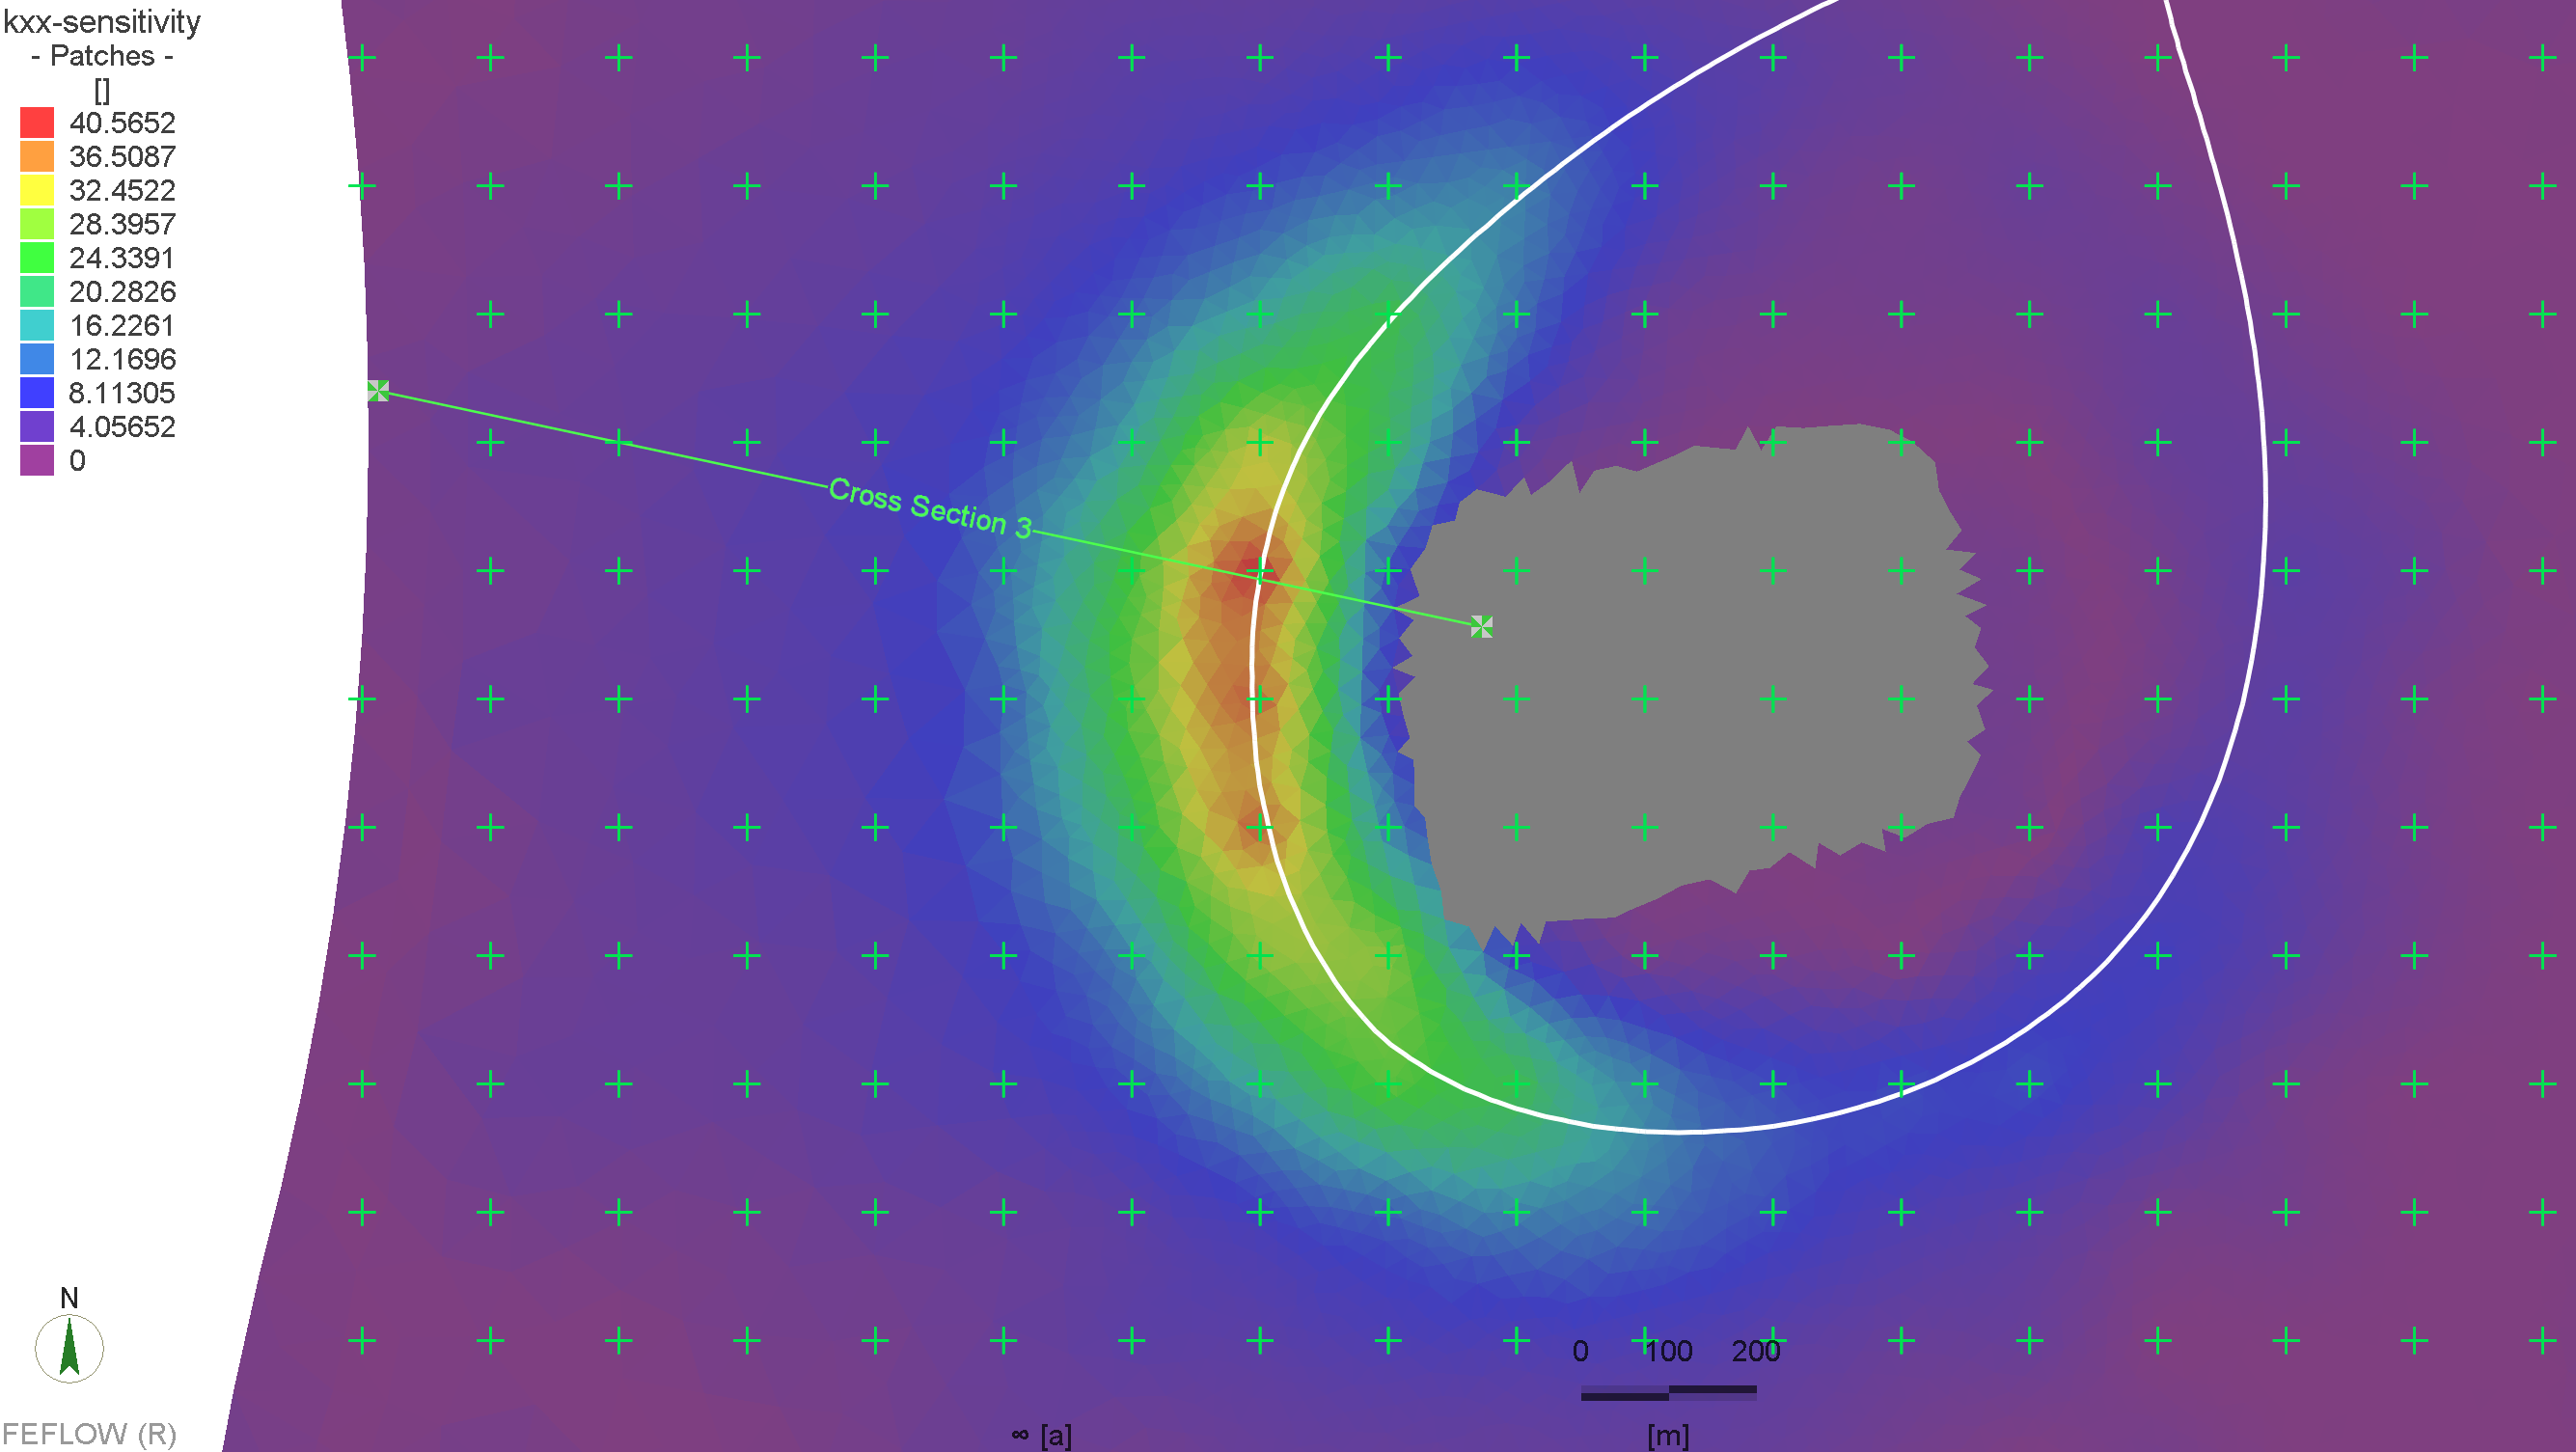
\includegraphics[width=\columnwidth]{figures/SensititivityExampleLayer5.png}
	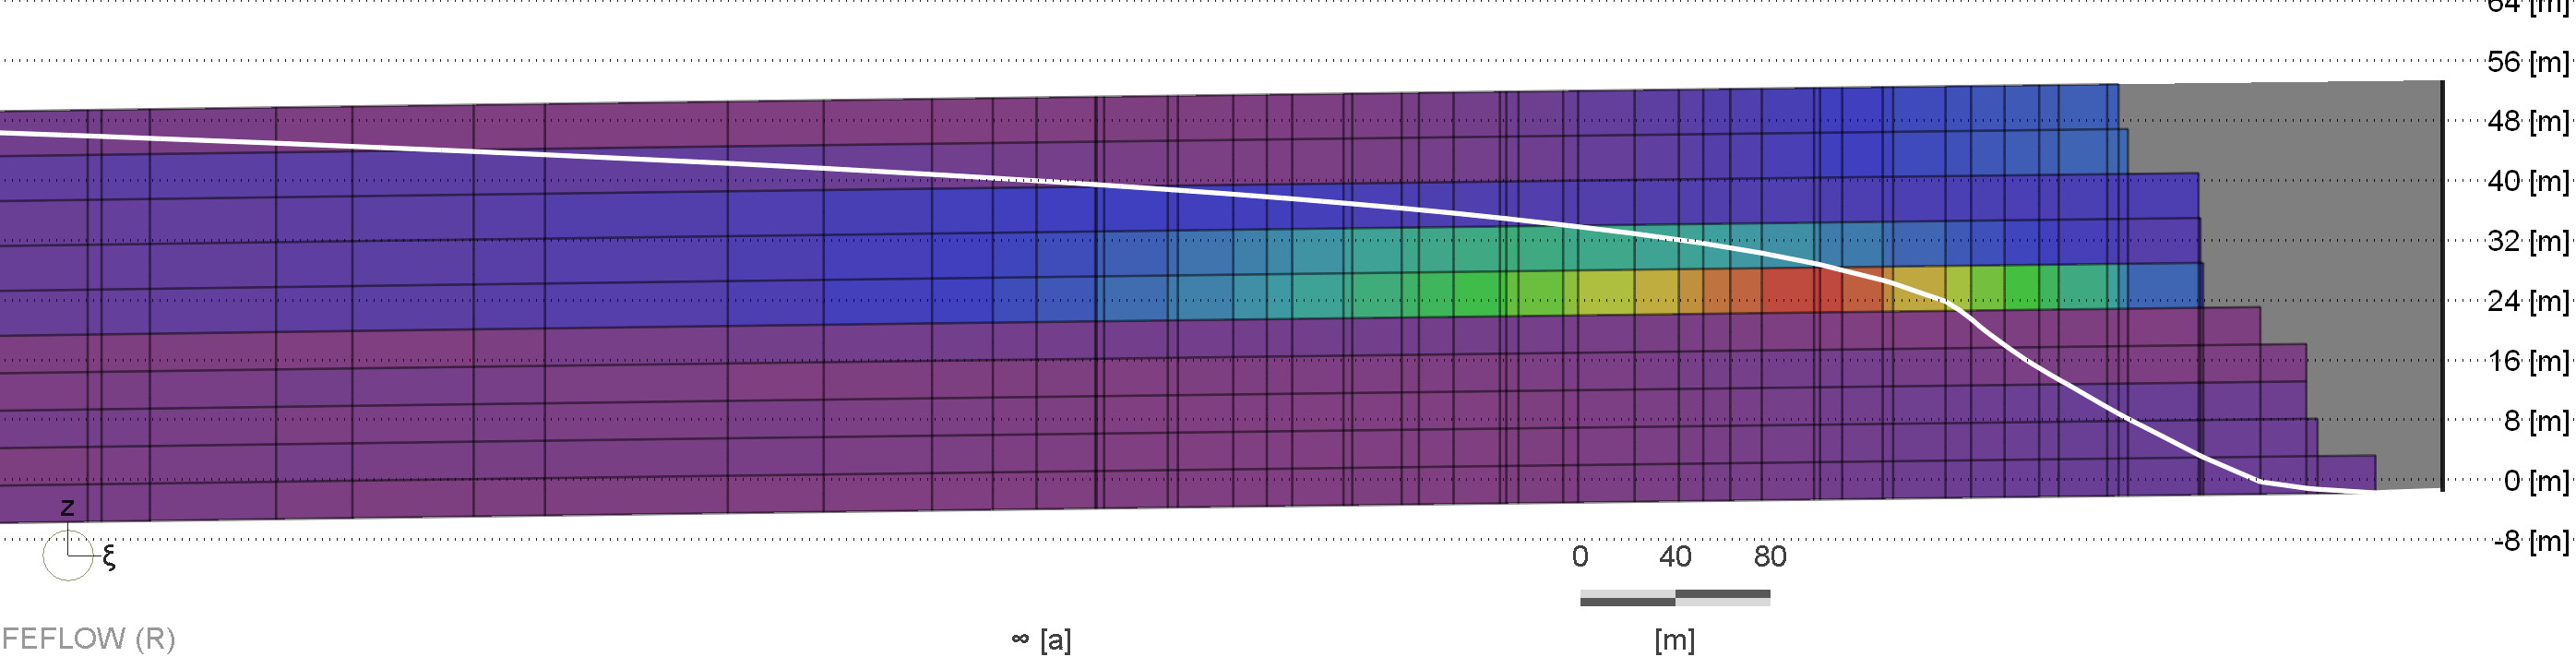
\includegraphics[width=\columnwidth]{figures/SensititivityExampleXSect.png}
\caption{Sensitivity maps (plain view of layer 5 and cross-section of indicated line shown.) of hydraulic conductivity in a 3D model. These are created by spatial interpolation of pilot point parameter sensitivity. White line indicates the water table.}
\label{fig:fepest:SensitivityMapMine}
\end{figure}

\section{Model Stability Tests (JACTEST)}
\label{sec:fepest:Jactest}

As discussed in section \ref{sec:fepest:derivativeCalculation}, it is important that the numerical model is stable enough to provide reproducible observation - parameter relationships. 

As a measure of trouble-shooting, PEST provides a tool (JACTEST) that checks if the model is running sufficiently stable to calculate the Jacobian matrix. This tool can be activated from within FePEST using the Model Stability option in the Estimation menu. 

JACTEST will run the model multiple times, each incrementing/decrementing the chosen parameter according to its settings for derivative calculation (see section \ref{sec:fepest:derivativeCalculation}) and plotting the response of the observations.

\textit{Further reading: Addendum to the PEST Manual (5th Ed.)
section 3.20: JACTEST and section \ref{sec:troubles:derivative} (p. \pageref{sec:troubles:derivative}) of this manual}


\subsection{Using JACTEST}

If PEST fails to reduce the objective function and bad derivative calculation is the suspected reason, stop PEST (if it is still running). Open the \textbf{Show Results} dialog and \textbf{Apply} the latest values as initial parameter values (you may want to save the FPS file now under a different name).

Open the Model stability dialog from the Estimation menu. The only settings required by the users are: 

\begin{itemize}
\item Specification of the parameters that are subject to the test. 

Those parameters that are suspected to cause instabilities should be chosen here.

\item Number of iterations to be performed on each parameter. 

PEST will increment/decrement the parameter this often. A value of 4 should be initially sufficient to identify parameter-observation relations that show a certain amounts of randomness.
\end{itemize}

After the calculation has finished, the diagram window shows the resulting observation values. If the slopes are similar or change gradually and monotonously, no problems are indicated. An example for a stable model is shown in Figure \ref{fig:fepest:jactestResult}.

\begin{figure}
	\center
	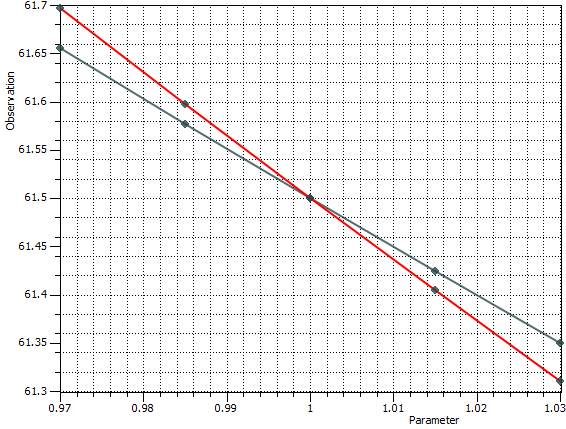
\includegraphics[width=\columnwidth]{figures/jactestResult.png}
\caption{JACTEST result indicating stable model behavior. Two parameters are incremented / decremented four times each by 1.5~\% around the initial value, the resulting values for a particular hydraulic head observation are plotted.}
\label{fig:fepest:jactestResult}
\end{figure}

If the parameter values change randomly (and significantly) or contain discontinuities noise dominates the observation. Identify the affected parameter-observation combinations, and open and run the model in FEFLOW to find and solve the instability issue.